\section{Distribución}
\label{sec:distribucion}
Se introduce a continuación la forma en que se divulga el proyecto \textit{VSCode4Teaching} en sus distintas etapas: tanto como código fuente (\referenciaSeccion{subsec:distribFuente}) como los artefactos construidos de la extensión y el servidor con la aplicación web (\referenciaSeccion{subsec:distribArtefactos}).

\subsection{Distribución del código fuente}
\label{subsec:distribFuente}
El código fuente del proyecto \textit{VSCode4Teaching} se encuentra íntegramente publicado en la red a través de un repositorio alojado en GitHub (\referenciaSeccion{subsec:tecGitHub}), tal como ilustra la \referenciaFigura{fig:distribGitHub}.

\begin{figure}[ht]
    \centering
    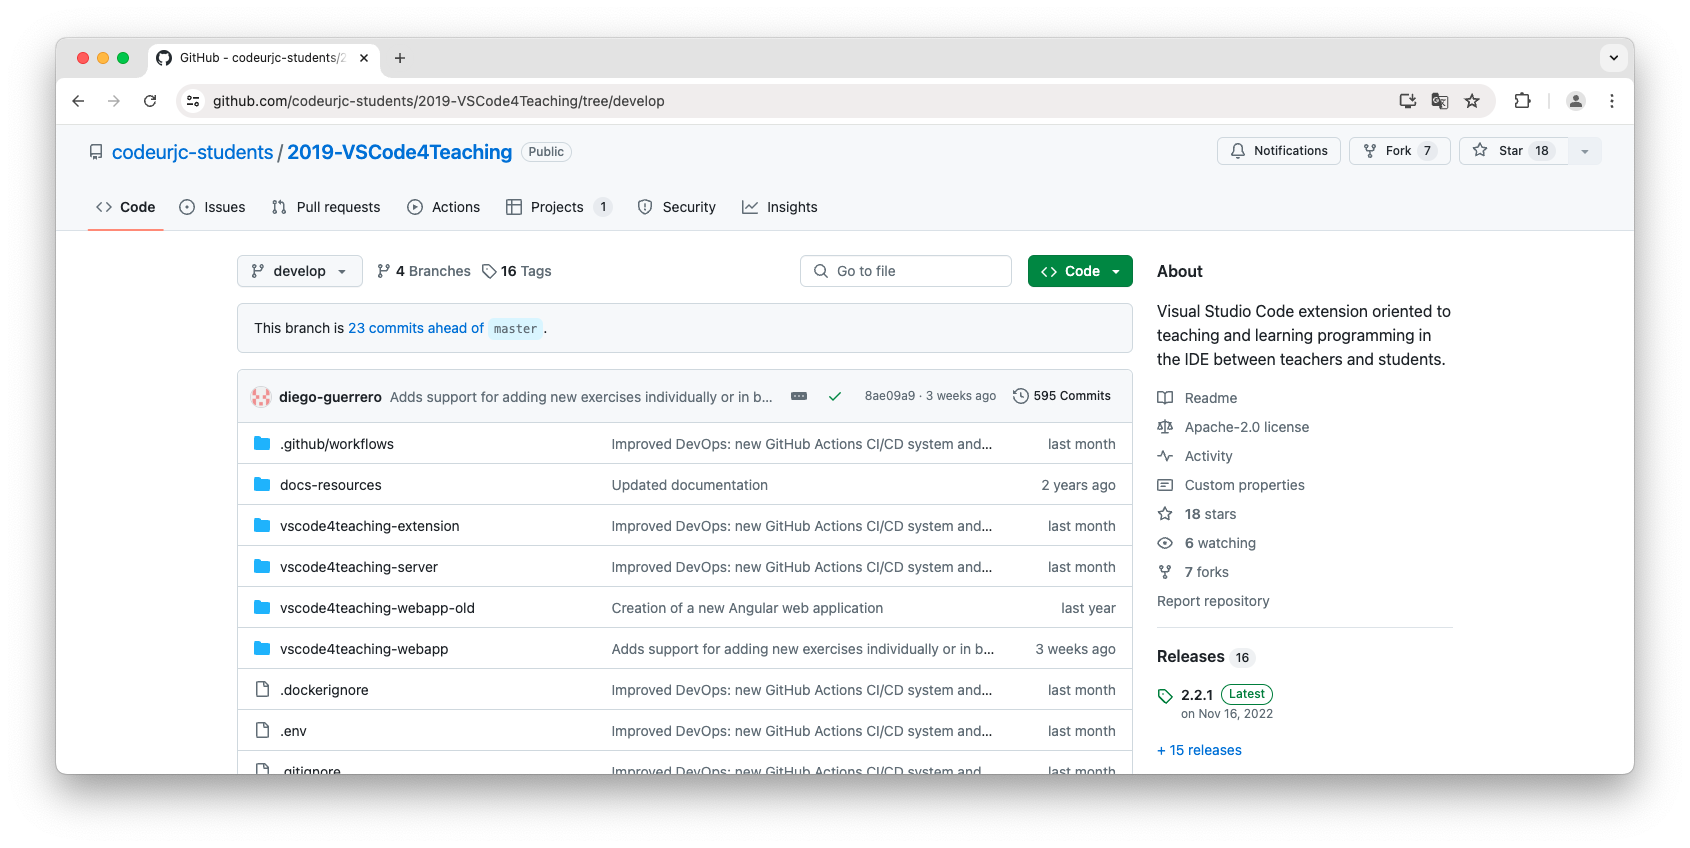
\includegraphics[width=0.8\linewidth]{imagenes/utilizadas/4-5-distribucion/repoGitHub.png}
    \caption{Repositorio en GitHub del proyecto \textit{VSCode4Teaching}.}
    \label{fig:distribGitHub}
\end{figure}

Este repositorio viene utilizándose desde el inicio del proyecto y contiene el histórico completo de cambios producidos en la aplicación durante su evolución. Se encuentra alojado en la siguiente dirección:

\vspace{-0.7\baselineskip}
\begin{center}
    \href{https://github.com/codeurjc-students/2019-VSCode4Teaching}{https://github.com/codeurjc-students/2019-VSCode4Teaching}.
\end{center}
\vspace{-0.7\baselineskip}

Tal como incluye en el fichero \texttt{LICENSE} alojado en su raíz, el código fuente de \textit{VSCode4Teaching} está sujeto a la licencia Apache License 2.0 \cite{ApacheLicense}. Esta licencia es permisiva y permite a otros desarrolladores utilizar el código del proyecto para su modificación y redistribución libremente siempre y cuando se mantenga la licencia sobre todas aquellas partes del fuente que no hayan sido adaptadas en las nuevas versiones generadas.

Esta licencia permite, además, aseverar que \textit{VSCode4Teaching} es \textit{software} libre, ya que otorga a sus usuarios las cuatro libertades esenciales: libertad de ejecutarlo como se desee y para lo que se desee, libertad de estudiar cómo funciona y poder adaptarlo para modificar su comportamiento, libertad para redistribuirlo y libertad para distribuir también las copias modificadas \cite{FreeSoftwareFreedoms}.

\subsection{Distribución de artefactos}
\label{subsec:distribArtefactos}
Además de la distribución de su código fuente, el proyecto \textit{VSCode4Teaching} publica sus artefactos empaquetados para una utilización directa más sencilla de la aplicación. Tal como se introduce en la \referenciaSeccion{subsec:tecDistrib}, se hace uso de dos repositorios públicos para la divulgación de la extensión para Visual Studio Code y del servidor empaquetado junto con la aplicación web en una imagen Docker (véase el requisito \referenciaConTT{subsec:rn4}{RN-4}).

La extensión queda publicada mediante el sistema de integración continua (véase el requisito \referenciaConTT{subsec:rn5}{RN-5}) en el Visual Studio Code Marketplace, lo que posibilita que esté disponible directamente para los usuarios a través de la herramienta integrada para la búsqueda e instalación de extensiones, tal como muestra la \referenciaFigura{fig:distribVSCodeMarketplace}.
\begin{figure}[ht]
    \centering
    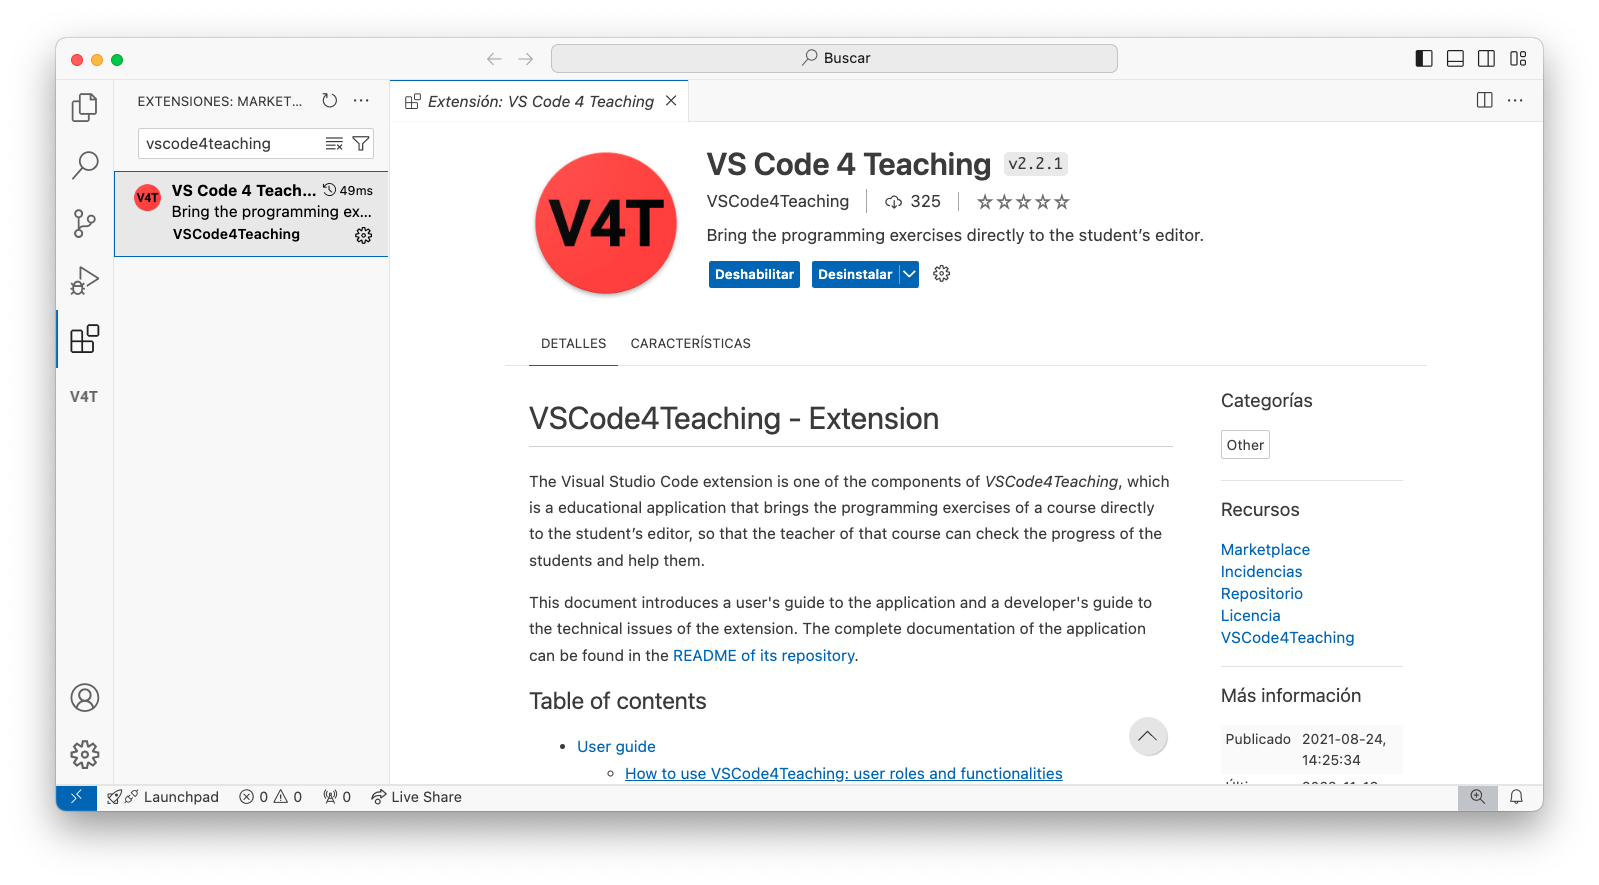
\includegraphics[width=0.8\linewidth]{imagenes/utilizadas/4-5-distribucion/vscodeMarketplace.png}
    \caption{Extensión de \textit{VSCode4Teaching} en el área de búsqueda y descarga de extensiones en Visual Studio Code.}
    \label{fig:distribVSCodeMarketplace}
\end{figure}

\noindent El enlace a la extensión publicada es el siguiente:
\vspace{-0.7\baselineskip}
\begin{center}
    \href{https://marketplace.visualstudio.com/items?itemName=VSCode4Teaching.vscode4teaching}{https://marketplace.visualstudio.com/items\\ ?itemName=VSCode4Teaching.vscode4teaching}.
\end{center}
\vspace{-0.7\baselineskip}

Por otro lado, el servidor queda empaquetado junto con la aplicación web como \textit{frontend} en una imagen Docker generada mediante el sistema de CI/CD que queda publicada en el Docker Hub, tal como se detalla en los requisitos \referenciaConTT{subsec:rn4}{RN-4} (acerca de la generación) y \referenciaConTT{subsec:rn5}{RN-5} (sobre la automatización), quedando disponible para su utilización mediante, por ejemplo, el fichero \textit{docker-compose.yml} disponible en el repositorio.

\noindent El enlace a la imagen publicada del servidor con la aplicación web es el siguiente:
\vspace{-0.7\baselineskip}
\begin{center}
    \href{https://hub.docker.com/r/vscode4teaching/vscode4teaching}{https://hub.docker.com/r/vscode4teaching/vscode4teaching}.
\end{center}
\vspace{-0.7\baselineskip}
